\documentclass[compress]{beamer}

\usetheme{Szeged}

\usepackage[T1]{fontenc}
\usepackage[utf8]{inputenc}
\usepackage[frenchb]{babel}
\usepackage[babel=true,kerning=true]{microtype}
\usepackage{tikz,listings,algorithm,algorithmic,hyperref,footbib}
\usepackage{xmpmulti,pgfbaseplot,lmodern}

\usetikzlibrary{automata,shapes,snakes,arrows,petri,decorations,backgrounds,shadows}
\usetikzlibrary{fadings,patterns,calc,fit,chains,positioning,scopes}
\tikzstyle{every picture}=[sibling distance=3cm, shorten >=1pt, node distance=2cm,%
	>=stealth', bend angle=10, auto, initial text=]
\tikzstyle{active}=[draw=blue!50, fill=blue!20]
\tikzstyle{failure}=[draw=black!50, fill=black!20]

\title[SEM AU311 - Suivi de Situation]{{\Large Suivi de Situation}\\AU311 - Opération et Supervision}
\author[Charles Lesire]{Charles Lesire-Cabaniols (ONERA / DCSD)\\{\tt charles.lesire@onera.fr}}
\date[2010-2011]{3A-SEM - 2010-2011}

\graphicspath{{../figures/},{../figures/suivi/}}
\lstset{basicstyle=\tiny,tabsize=2,%frame=single,%
	emph={define,domain,requirements,strips,typing,types,predicates,
		action,parameters,precondition,vars,effect,objects,init,goal},%
	emphstyle=\bf}

%\footbibliographystyle{alpha}
%\footbibliography{../biblio}

\begin{document}

\begin{frame}
\titlepage
\end{frame}

\begin{frame}
\tableofcontents[hidesubsections]
\end{frame}

%%%% INTRODUCTION %%%%
\section{Introduction}

\begin{frame}
\tableofcontents[currentsection,hideothersubsections]
\end{frame}

\subsection{Autonomie}
\begin{frame}{Autonomie}{Fonctions nécessaires}
\begin{itemize}
\item Avant la mission : 
	\begin{itemize}
	\item Planification (véhicule)
	\item Procédures (opérateur)
	\end{itemize}
\item En opération :
	\begin{itemize}
	\item Supervision
	\item (Re)Planification
	\item Gestion des communications
	\item Interfaces opérateur
	\item \structure{Suivi de l'état}
	\end{itemize}
\end{itemize}
\end{frame}

%\begin{frame}{Autonomie}{La {\it double boucle}}
%\end{frame}

\subsection{Suivi de l'état}
\begin{frame}{Suivi de l'état}{C'est quoi ?}
\begin{itemize}
\item Suivi de l'état du véhicule
\item Suivi de l'état de l'environnement
\item Détection de pannes
\item Diagnostic
\item \'Evaluation de la situation
\item Conscience de la situation
\item Prédiction
\end{itemize}
\end{frame}

\begin{frame}{Conscience de situation}
\begin{quote}
Situation awareness involves being aware of what is happening
around you to understand how information, events, and your own
actions will impact goals and objectives, both now and in the near
future.
\end{quote}
\end{frame}

\begin{frame}{Suivi de l'état}{Pouquoi faire ?}
\begin{itemize}
\item Pour :
	\begin{itemize}
	\item Décider
	\item Réagir, Alerter
	\item Replanifier, Reconfigurer
	\end{itemize}
\item Sur la base :
	\begin{itemize}
	\item des tâches, activités, procédures
	\item de l'état de santé du véhicule
	\item des ressources disponibles (dont communication)
	\item de l'état de l'environnement
	\item des actions de l'opérateur
	\end{itemize}
\end{itemize}
\end{frame}

\begin{frame}{Conscience de situation}
\begin{center}
	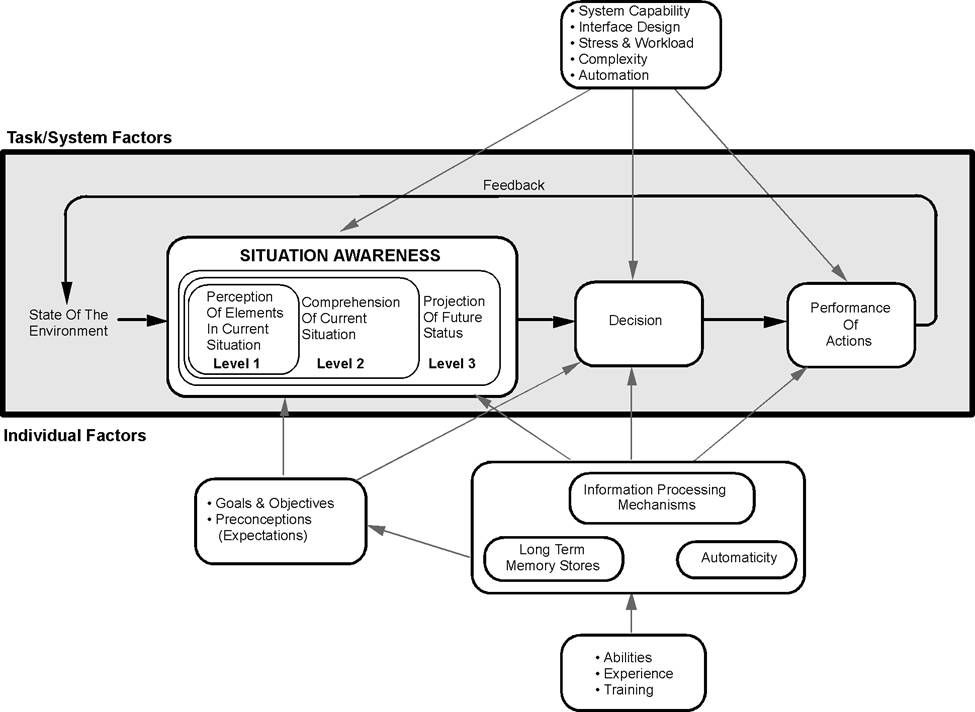
\includegraphics[width=.7\linewidth]{SA-Endsley}\\
	Place du Suivi de Situation chez l'opérateur (Endsley, 1995)
\end{center}
\end{frame}

\subsection{Suivi de situation}
\begin{frame}{Suivi de situation}
\begin{itemize}
\item Situation Awareness : {\it conscience de la situation (par l'opérateur)}
\item \structure{Situation Assessment} : {\it élaboration, évaluation de la situation (algorithmique)}
\item 3 niveaux :
	\begin{enumerate}
	\item \structure{Perception} : acquisition des informations pertinentes,
		reconnaissance de situations élémentaires ;
	\item \structure{Compréhension} : synthèse des situations perçues, 
		interprétation par rapport aux modèles (environnement, tâches, procédures) ;
	\item \structure{Projection} : prédiction de l'impact des actions
		 en fonction de la situation	 et des modèles.
	\end{enumerate}
\end{itemize}
\end{frame}

\begin{frame}{Niveaux de situation (Waltz, 2000)}
\begin{center}
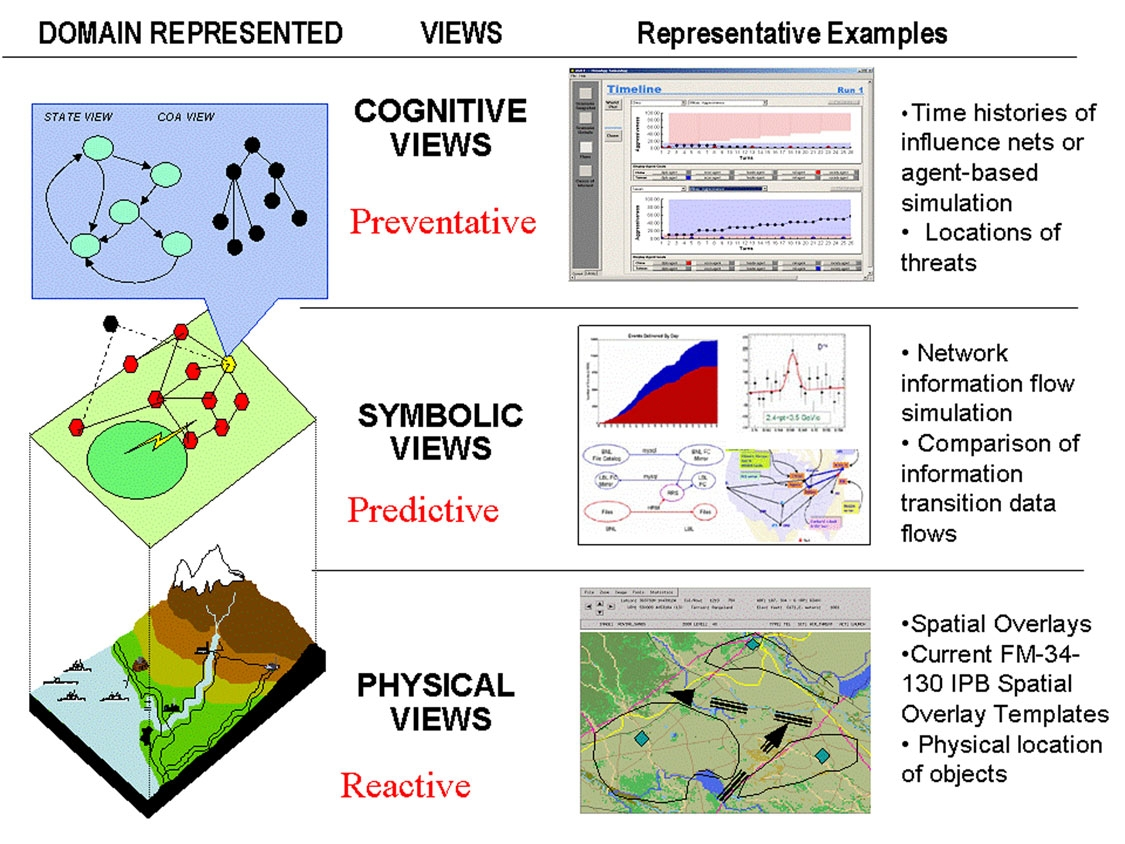
\includegraphics[width=.7\linewidth]{nvx-situation}
\end{center}
\end{frame}

\subsection{Systèmes continus}
\begin{frame}{Approche \it systèmes continus}
\begin{columns}
\begin{column}{.65\linewidth}
	\begin{itemize}
	\item Filtrage bayésien : estimation des variables d'un système soumis à des perturbations\\
		{\it Filtre de Kalman et ses extensions}
	\item Filtrage particulaire : estimation de l'état par sélection des particules les plus cohérentes 
		avec les observations
	\end{itemize}
\end{column}
\begin{column}{.3\linewidth}
	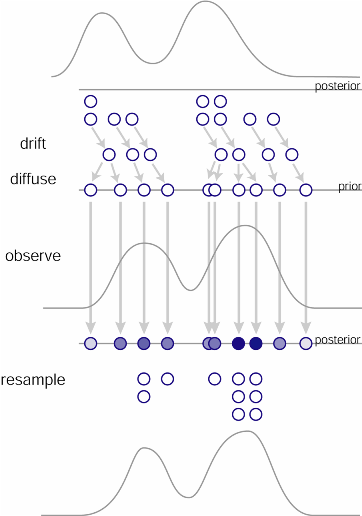
\includegraphics[width=\linewidth]{pf}
\end{column}
\end{columns}
\end{frame}

%%%%% SYSTEMES DISCRETS %%%%%
\section{Systèmes à événements discrets}

\begin{frame}
\tableofcontents[currentsection,hideothersubsections]
\end{frame}

\subsection{Introduction}
\begin{frame}{Approche \it systèmes à événements discrets}
\begin{itemize}
\item Représentation symbolique de l'état du système\\
	Ex. : {\it "le piéton se dirige vers le véhicule"}\\
	\qquad {\it "PA en mode \bf climb"}
\item \'Etats, transitions, contraintes, incertitudes
\item Mise en correspondance des observations avec le modèle
\end{itemize}
\end{frame}

\subsection{Chroniques}
\begin{frame}{Chroniques}{Définitions}
\begin{itemize}
\item Modélisation d'une activité, d'une tâche, d'un comportement... sous forme de contraintes temporelles entre événements ;
\item Algorithme de reconnaissance d'une activité à partir des événements perçus.
\item \url{http://crs.elibel.tm.fr/}
\end{itemize}
\end{frame}

\begin{frame}{Chroniques}{Définitions}
\begin{block}{Chronique (Dousson {\it et al.}, 1993)}
Un modèle de chronique $C$ est un couple $(S, T)$ avec
\begin{itemize}
\item $S$ un ensemble d'événements
\item $T$ l'ensemble des contraintes entre les instants de ces événements.
\end{itemize}
\end{block}
\end{frame}

\begin{frame}[fragile]{Chroniques}{Exemple (Vu Duong, 2001)}
\begin{columns}
\begin{column}{0.45\linewidth}
\begin{tikzpicture}
\node[draw, inner sep=3pt] (c) at (0:1.5) {$C$};
\node[draw, inner sep=3pt] (b) at (90:1.5) {$B$} edge[->] node[above, right] {$[1, 1]$} (c);
\node[draw, inner sep=3pt] (a) at (180:1.5) {$A$} edge[->] node[above, left] {$[2, 4]$} (b)
						edge[->] node[below] {$[3, 5]$} (c);
\end{tikzpicture}
\end{column}
\begin{column}{0.45\linewidth}
\begin{verbatim}
chronicle Ch {
   event(A, ta);
   event(B, tb);
   event(C, tc);

   tb - ta in [2, 4];
   tc - ta in [3, 5];
   tc - tb in [1, 1];
}
\end{verbatim}
\end{column}
\end{columns}
\end{frame}

\begin{frame}{Reconnaissance de Chroniques}
\begin{center}
\begin{tikzpicture}[scale=.9,transform shape]
%% L'arbre
\path node[draw, inner xsep=5pt] (1) {1}
	child {node[draw, inner xsep=5pt] (2) {2}
		child {node[draw, inner xsep=5pt] (3) {3}
			child {node[draw, inner xsep=5pt] (5) {5}}}}
	child {node[draw, inner xsep=5pt] (4) {4}};
%% Timeline 1
\path[draw, dashed, ->, overlay]<+-> (1) -- ++(3, 0) node[draw, dashed, anchor=west] {%
	\tikzpicture[solid,-,x=1cm,y=1.5cm]
	\draw (0,0) -- +(0,1)
	{[left=3pt, baseline] node[pos=.2] {\tiny C} node[pos=.5] {\tiny B} node[pos=.8] {\tiny A}}
	node[above] {\tiny 0}
	+(1,0) -- +(1,1) node[above] {\tiny $\infty$};
	\draw[color=blue!50, ultra thick] (0,0)
	+(0,.2) -- +(1,.2)
	+(0,.5) -- +(1,.5)
	+(0,.8) -- +(1,.8);
	\endtikzpicture};
%% Timeline 2
\path[draw, dashed, ->, overlay]<+-> (2) -- ++(-2, 1.5) node[draw, dashed, anchor=east] {%
	\tikzpicture[solid,-,x=0.25cm,y=1.5cm]
	\draw (0,0) -- +(0,1)
	{[left=3pt, baseline] node[pos=.2] {\tiny C} node[pos=.5] {\tiny B} node[pos=.8] {\tiny A}}
	node[above] {\tiny 1}
	+(1,0) -- +(1,1) node[above] {\tiny 3}
	+(2,0) -- +(2,1) node[above] {\tiny 4}
	+(3,0) -- +(3,1) node[above] {\tiny 5}
	+(4,0) -- +(4,1) node[above] {\tiny 6};
	\draw[color=blue!50, ultra thick] (0,0)
	+(2,.2) -- +(4,.2)
	+(1,.5) -- +(3,.5);
	\fill[color=red] +(0,.8) circle (.5mm);
	\endtikzpicture} node[above=3pt, pos=.3] {\footnotesize $(A, 1)$};
%% Timeline 3
\path[draw, dashed, ->, overlay]<+-> (3) -- ++(1.5, -.5) node[draw, dashed, anchor=west] {%
	\tikzpicture[solid,-,x=0.33cm,y=1.5cm]
	\draw (0,0) -- +(0,1)
	{[left=3pt, baseline] node[pos=.2] {\tiny C} node[pos=.5] {\tiny B} node[pos=.8] {\tiny A}}
	node[above] {\tiny 1}
	+(1,0) -- +(1,1) node[above] {\tiny 3}
	+(2,0) -- +(2,1) node[above] {\tiny 4};
	\draw[color=blue!50, ultra thick] (0,0)
	+(1.8,.2) -- +(2.2,.2);
	\fill[color=red]
	+(0,.8) circle (.5mm)
	+(1,.5) circle (.5mm);
	\endtikzpicture} node[above=3pt, pos=.3] {\footnotesize $(B, 3)$};
%% Timeline 4
\path[draw, dashed, ->, overlay]<+-> (4) -- ++(2.5, -1.5) node[draw, dashed, anchor=west] {%
	\tikzpicture[solid,-,x=0.25cm,y=1.5cm]
	\draw (0,0) -- +(0,1)
	{[left=3pt, baseline] node[pos=.2] {\tiny C} node[pos=.5] {\tiny B} node[pos=.8] {\tiny A}}
	node[above] {\tiny 4}
	+(1,0) -- +(1,1) node[above] {\tiny 6}
	+(2,0) -- +(2,1) node[above] {\tiny 7}
	+(3,0) -- +(3,1) node[above] {\tiny 8}
	+(4,0) -- +(4,1) node[above] {\tiny 9};
	\draw[color=blue!50, ultra thick] (0,0)
	+(2,.2) -- +(4,.2)
	+(1,.5) -- +(3,.5);
	\fill[color=red] +(0,.8) circle (.5mm);
	\endtikzpicture} node[above=3pt, pos=.3] {\footnotesize $(A, 4)$};
%% Timeline 5
\path[draw, dashed, ->, overlay]<+-> (5) -- ++(-2, .8) node[draw, dashed, anchor=east] {%
	\tikzpicture[solid,-,x=0.33cm,y=1.5cm]
	\draw (0,0) -- +(0,1)
	{[left=3pt, baseline] node[pos=.2] {\tiny C} node[pos=.5] {\tiny B} node[pos=.8] {\tiny A}}
	node[above] {\tiny 1}
	+(1,0) -- +(1,1) node[above] {\tiny 3}
	+(2,0) -- +(2,1) node[above] {\tiny 4};
	\fill[color=red]
	+(0,.8) circle (.5mm)
	+(1,.5) circle (.5mm)
	+(2,.2) circle (.5mm);
	\endtikzpicture} node[above=3pt, pos=.3] {\footnotesize $(C, 4)$};
\end{tikzpicture}
\end{center}
\end{frame}

\begin{frame}{Reconnaissance de Chroniques}
\begin{itemize}
\item Propagation de contraintes,
\item Factorisation de l'arbre,
\item Notion de "sous-chronique".
\item Méthodes d'apprentissage de chroniques...
\item Application à la détection de fautes dans les réseaux de télécommunications.
\end{itemize}
\end{frame}

\begin{frame}{Diagnostic d'arythmies cardiaques (Quiniou {\it et al.}, 2008)}
\begin{columns}
\begin{column}{0.55\linewidth}
\begin{center}
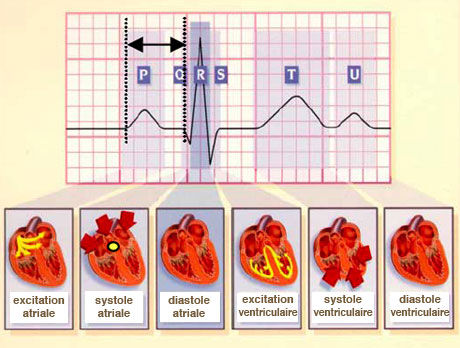
\includegraphics[width=0.9\linewidth]{schemaECG}\\
\small Contraction cardiaque et ECG
\end{center}
\end{column}
\begin{column}{0.45\linewidth}
\begin{center}
\centering 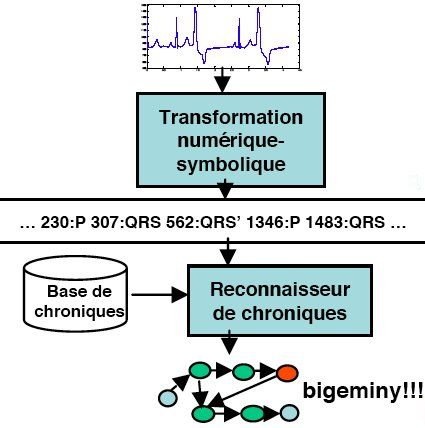
\includegraphics[width=0.9\linewidth]{reconnaisseur}\\
\small Principe de reconnaissance de pathologies
\end{center}
\end{column}
\end{columns}
\end{frame}

\begin{frame}{Diagnostic d'arythmies cardiaques (Quiniou {\it et al.}, 2008)}
\begin{center}
\multiinclude[<+>][format=png,graphics={height=6.5cm}]{recoVB}
\end{center}
\end{frame}

\begin{frame}{Reconnaissance d'activités sur vidéos (Rota et Thonnat, 2000)}
\begin{center}
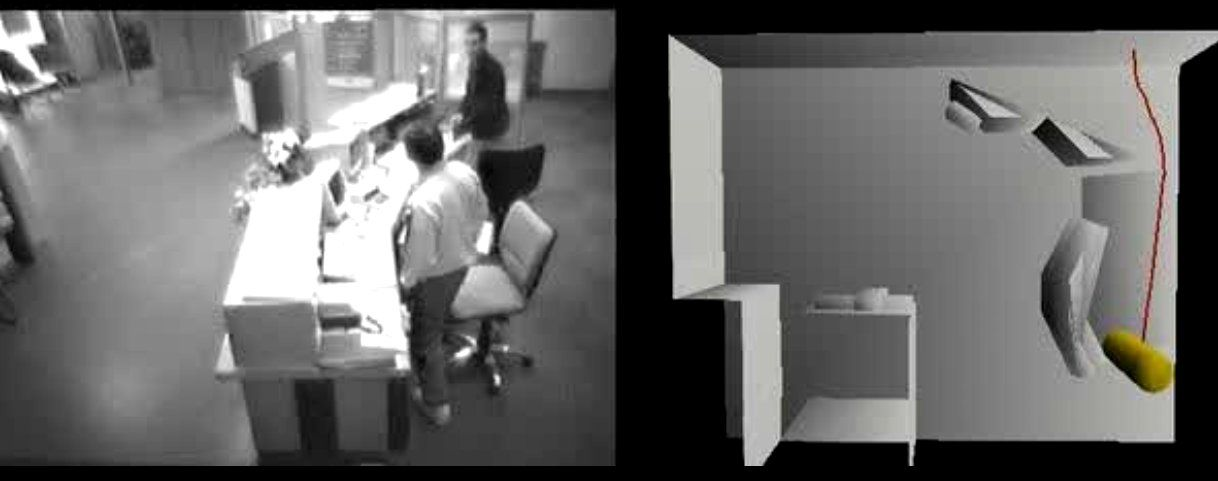
\includegraphics[width=0.9\linewidth]{reco-banque}\\
%\movie[showcontrols]{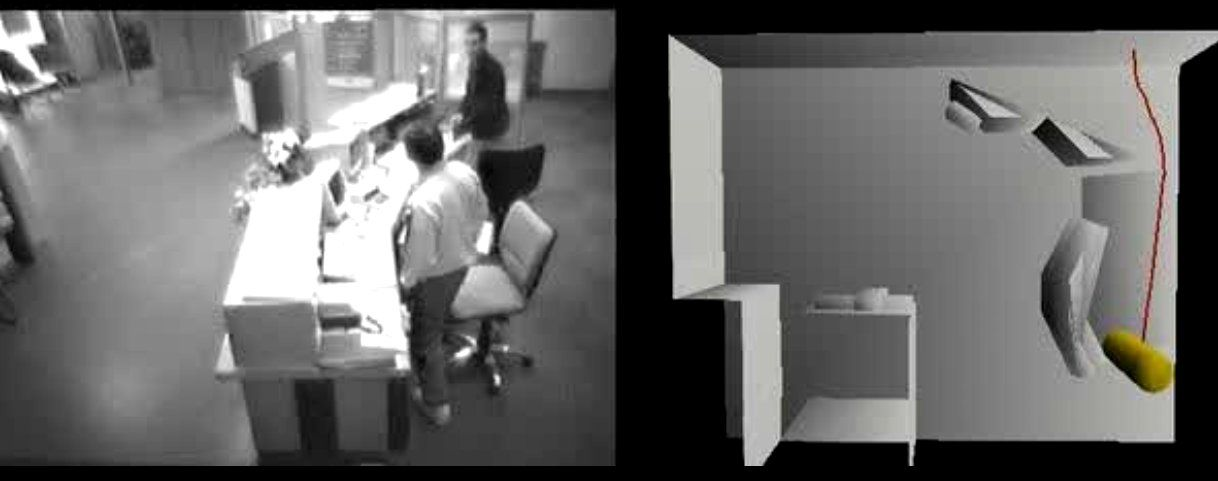
\includegraphics[width=0.9\linewidth]{reco-banque}}{\thevideo/mc2-17_reals2.mpeg}\\
\small Reconnaissance d'une scène de prise d'hotage dans une banque
\end{center}
\end{frame}

%%%% AUTOMATES %%%%%
\subsection{Automates}
\begin{frame}{Automates}
\begin{itemize}
\item Approche "systémique",
\item Modélisation du comportement,
\item Utilisation des événements pour "jouer" l'automate.
\end{itemize}
\end{frame}

\begin{frame}{Automates}{Définition}
\begin{block}{Automate}
Un \structure{automate} est un 4-uplet $A=(\Sigma, Q, Q_0, T)$~:
\begin{itemize}
\item $\Sigma$ est un alphabet fini,
\item $Q$ est l'ensemble des places (états, lieus, localités),
\item $Q_0$ est l'ensemble des places initiales,
\item $T \subset Q \times Sigma \times Q$ est la fonction de transition.
\end{itemize}
$e = <q, a, q'>$ est une transition de la place $q$ vers la place $q'$ étiquetée par la lettre $a$.
\end{block}
\end{frame}

\begin{frame}{Automates}{Exemple}
\begin{center}
\begin{tikzpicture}
\path node[state, initial] (q_0) {$q_0$};
\path node[state] (q_1) [right of=q_0] {$q_1$};
\path node[state] (q_2) [right of=q_1] {$q_2$};
\path node[state, accepting] (q_3) [right of=q_2] {$q_3$};
\path[->] (q_0) edge[loop above] node {\alert<2>{$b$}} ();
\path[->] (q_0) edge[bend left] node {\alert<3,5>{$a$}} (q_1);
\path[->] (q_1) edge[bend left] node {\alert<4>{$b$}} (q_0);
\path[->] (q_1) edge node {\alert<6>{$a$}} (q_2);
\path[->] (q_2) edge[loop above] node {$a$} ();
\path[->] (q_2) edge node {\alert<7>{$b$}} (q_3);
\path[->] (q_3) edge[bend angle=25, bend left] node {$a$} (q_1);
\path[->] (q_3) edge[bend angle=45, bend left] node {$b$} (q_0);
% Overlays
\path[overlay]<1,2,4|handout:0> node[state, initial, active] (q_0) {$q_0$};
\path[overlay]<3,5|handout:0> node[state, active] (q_1) [right of=q_0] {$q_1$};
\path[overlay]<6|handout:0> node[state, active] (q_2) [right of=q_1] {$q_2$};
\path[overlay]<7|handout:0> node[state, accepting, active] (q_3) [right of=q_2] {$q_3$};
\end{tikzpicture}
\end{center}
$\Sigma \; \longleftarrow \quad %
	\alert<2>{b} \; \alert<3>{a} \; \alert<4>{b} \; \alert<5>{a} \; \alert<6>{a} \; \alert<7>{b}$
\end{frame}

\begin{frame}{Automates}{Non-déterminisme}
\begin{block}{Non-déterminisme}
\begin{itemize}
\item \'Evénements non-observables (ex. : pannes),
\item Effets non-déterministes,
\item Différentes modélisation (\alert<2->{ensembliste}, probabiliste, floue\dots)
\end{itemize}
\end{block}
\end{frame}

\begin{frame}{Automates}{Non-déterminisme}
\begin{center}
\begin{tikzpicture}[scale=.8, transform shape, node distance=1.5cm]
\path node[state, initial] (q_0) {$q_0$};
\path node[state] (q_1) [right of=q_0] {$q_1$};
\path node[state] (q_2) [above right of=q_1] {$q_2$};
\path node[state] (q_3) [below right of=q_1] {$q_3$};
\path node[state] (q_4) [right of=q_2] {$q_4$};
\path node[state] (q_5) [right of=q_3] {$q_5$};
\path node[state] (q_6) [below right of=q_4] {$q_6$};
\path node[state] (q_7) [right of=q_6] {$q_7$};
\path node[state] (q_8) [right of=q_7] {$q_8$};
\path node[state] (q_9) [right of=q_8] {$q_9$};
\path node[state, accepting] (q_10) [right of=q_9] {$q_{10}$};
%% Edges
\path[->] (q_0) edge node {\alert<2>{$\epsilon$}} (q_1);
\path[->] (q_0) edge[bend angle=60, bend right] node {\alert<2>{$\epsilon$}} (q_7);
\path[->] (q_1) edge node {\alert<2,4,6,8,10,12>{$\epsilon$}} (q_2);
\path[->] (q_1) edge node {\alert<2,4,6,8,10,12>{$\epsilon$}} (q_3);
\path[->] (q_2) edge node {\alert<5,9,11>{$a$}} (q_4);
\path[->] (q_3) edge node {\alert<3,7,13>{$b$}} (q_5);
\path[->] (q_4) edge node {\alert<6,10,12>{$\epsilon$}} (q_6);
\path[->] (q_5) edge node {\alert<4,8>{$\epsilon$}} (q_6);
\path[->] (q_6) edge node {\alert<4,8,10,12>{$\epsilon$}} (q_7);
\path[->] (q_6) edge[looseness=1.4, bend angle=90, bend right] node[swap] {\alert<4,6,8,10,12>{$\epsilon$}} (q_1);
\path[->] (q_7) edge node {\alert<5,9,11>{$a$}} (q_8);
\path[->] (q_8) edge node {\alert<11>{$a$}} (q_9);
\path[->] (q_9) edge node {\alert<13>{$b$}} (q_10);
%% Overlays
\path[overlay]<1-2|handout:0> node[state, initial, active] (q_0) {$q_0$};
\path[overlay]<2,4,6,8,10,12|handout:0> node[state, active] (q_1) [right of=q_0] {$q_1$};
\path[overlay]<2,4,6,8,10,12|handout:0> node[state, active] (q_2) [above right of=q_1] {$q_2$};
\path[overlay]<2,4,6,8,10,12|handout:0> node[state, active] (q_3) [below right of=q_1] {$q_3$};
\path[overlay]<5-6,9-10,11-12|handout:0> node[state, active] (q_4) [right of=q_2] {$q_4$};
\path[overlay]<3-4,7-8,13|handout:0> node[state, active] (q_5) [right of=q_3] {$q_5$};
\path[overlay]<4,6,8,10,12|handout:0> node[state, active] (q_6) [below right of=q_4] {$q_6$};
\path[overlay]<2,4,8,10,12|handout:0> node[state, active] (q_7) [right of=q_6] {$q_7$};
\path[overlay]<5-6,9-10,11-12|handout:0> node[state, active] (q_8) [right of=q_7] {$q_8$};
\path[overlay]<11-12|handout:0> node[state, active] (q_9) [right of=q_8] {$q_9$};
\path[overlay]<13|handout:0> node[state, accepting, active] (q_10) [right of=q_9] {$q_{10}$};
\end{tikzpicture}
\end{center}
$\Sigma \; \longleftarrow \quad %
	\alert<3>{b} \; \alert<5>{a} \; \alert<7>{b} \; \alert<9>{a} \; \alert<11>{a} \; \alert<13>{b}$
\end{frame}

\begin{frame}{Automates}{Exemple : Détection de pannes}
\begin{center}
\begin{tikzpicture}[scale=.7, transform shape, node distance=2cm]
%% Nodes
\path node[state, initial] (q_0) {$q_0$};
\path node[state] (q_1) [right of=q_0] {$q_1$};
\path node[state] (q_2) [right of=q_1] {$q_2$};
\path node[state] (q_3) [below of=q_1] {$q_3$};
\path node[state] (q_4) [below of=q_3] {$q_4$};
\path node[state] (q_5) [below of=q_0] {$q_5$};
%% Edges
\path[->] (q_0) edge node {\alert<2>{$a$}} (q_1);
\path[->] (q_1) edge node {\alert<4>{$b$}} (q_2)
				edge[bend angle=60, bend left] node {\alert<3>{$\varepsilon_b$}} (q_4);
\path[->] (q_2) edge[bend angle=60, bend right] node[above] {\alert<5>{$\varepsilon_b$}} (q_0);
\path[->] (q_3) edge node {$a$} (q_5);
\path[->] (q_4) edge[bend angle=60, bend left] node {\alert<4>{$b$}} (q_5)
				edge node {\alert<3>{$\varepsilon_a$}} (q_3);
\path[->] (q_5) edge node {$a$} (q_1);
%% Initial
\path<1>[overlay] node[state, initial, active] (q_0) {$q_0$};
%% On recoit 'a'
\path<2-3>[overlay] node[state,active] (q_1) [right of=q_0] {$q_1$};
\path<3>[overlay] node[state,active] (q_3) [below of=q_1] {$q_3$};
\path<3>[overlay] node[state,active] (q_4) [below of=q_3] {$q_4$};
%% On recoit 'b'
\path<5->[overlay] node[state, initial, active] (q_0) {$q_0$};
\path<4->[overlay] node[state, active] (q_2) [right of=q_1] {$q_2$};
\path<4->[overlay] node[state, active] (q_5) [below of=q_0] {$q_5$};
\end{tikzpicture}\\
\small On reçoit les événements $a$ puis $b$ :\\
quels états possibles ? panne possible ?
\end{center}
\end{frame}

\begin{frame}{Automates}{Exemple : Rover martien (Williams {\it et al.}, 2004)}
\begin{center}
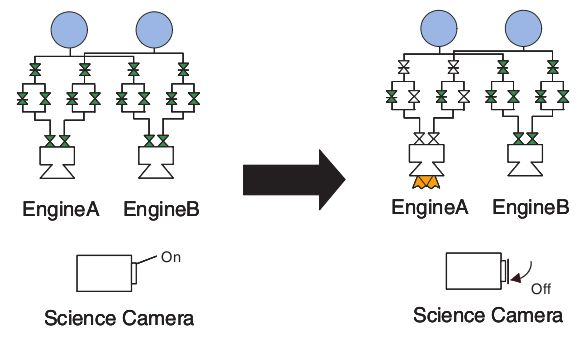
\includegraphics[width=0.6\linewidth]{engine}
\end{center}
\end{frame}

\begin{frame}{Automates}{Exemple : Rover martien (Williams {\it et al.}, 2004)}
\begin{columns}
\begin{column}{0.5\linewidth}
\centering
\begin{tikzpicture}[scale=.8, transform shape]
	\node[state] (q_off) {$q_0$};
	\node[state] (q_standby) [below of=q_off] {$q_1$};
	\node[state] (q_firing) [below of=q_standby] {$q_2$};
	\node[state, failure] (q_failed) [right of=q_standby] {$q_3$};
	\path[->] (q_off) edge [loop left] node {\bf Off} ()
			edge[bend angle=45, bend left] node {\footnotesize 0.01} (q_failed)
			edge[bend left] node {\footnotesize standby} (q_standby)
		(q_standby) edge [loop left] node {\bf Standby} ()
			edge node {\footnotesize 0.01} (q_failed)
			edge[bend left] node {\footnotesize off} (q_off)
			edge[bend left] node {\footnotesize fire} (q_firing)
		(q_firing) edge[loop left] node {\bf Firing} ()
			edge[bend angle=45, bend right] node[swap] {\footnotesize 0.01} (q_failed)
			edge[bend left] node {\footnotesize standby} (q_standby)
		(q_failed) edge[loop right] node {\bf Failed} ();
\end{tikzpicture}
\end{column}
\begin{column}{0.5\linewidth}
\centering
\begin{tikzpicture}[scale=.8, transform shape]
	\node[state] (q_off) {$q_0$};
	\node[state] (q_on) [below of=q_off] {$q_1$};
	\node[state, failure] (q_failed) [right of=q_off] {$q_2$};
	\path[->] (q_off) edge[loop left] node {\bf Off} ()
			edge node {\footnotesize 0.01} (q_failed)
			edge[bend left] node {\footnotesize on} (q_on)
		(q_on) edge[loop left] node {\bf On} ()
			edge[bend left] node {\footnotesize off} (q_off)
			edge[bend left] node[pos=.7] {\footnotesize 0.01} (q_failed)
		(q_failed) edge[loop right] node {\bf Failed} ()
			edge[bend left] node {\footnotesize reset} (q_on);
\end{tikzpicture}
\end{column}
\end{columns}
\begin{center}
\end{center}
\end{frame}

\begin{frame}{Automates}
\begin{itemize}
\item Modèle riche (extension temporelles, probabilistes\dots),
\item Estimation de l'état discret,
\item Détection de modes défaillants.
\end{itemize}
\end{frame}

%%%%% RESEAUX DE PETRI %%%%%
\subsection{Réseaux de Petri}

\begin{frame}{Kalmansymbo (Tessier, 2003)}
\begin{itemize}
\item Basé sur les réseaux de Petri,
\item Principe d'estimation récursif (prédiction/recalage),
\item Basé sur les similitudes entre propriétés.
\end{itemize}
\end{frame}

\begin{frame}{Kalmansymbo (Tessier, 2003)}
\begin{columns}[t]
\begin{column}{0.6\linewidth}
\begin{center}
\vspace{-1cm}
\begin{tikzpicture}[scale=0.45, transform shape, node distance=1.8cm]
%%%% Tikz Picture du rdP de Départ Vehicule
%% Petri net
\node[transition] (t1) {}; \node[node distance=12pt, left of=t1] {$t_1$};
\node[place, below of=t1] (c2) {}; \node[node distance=18pt, left of=c2] {$c_2$};
\node[place, left of=c2] (a2) {}; \node[node distance=18pt, below right of=a2] {$a_2$};
\node[place, right of=c2] (a1) {}; \node[node distance=18pt, left of=a1] {$a_1$};
\node[place, right of=a1] (c1) {}; \node[node distance=18pt, left of=c1] {$c_1$};
\node[transition, above of=c1] (t0) {}; \node[node distance=12pt, left of=t0] {$t_0$};
\node[transition, below of=a2] (t2) {}; \node[node distance=12pt, right of=t2] {$t_2$};
\node[transition, below of=c2] (t3) {}; \node[node distance=12pt, left of=t3] {$t_3$};
\node[place, below of=t2] (a3) {}; \node[node distance=18pt, right of=a3] {$a_3$};
\node[place, below right of=t3] (a4) {}; \node[node distance=18pt, left of=a4] {$a_4$};
\node[transition, below right of=a4] (t4) {}; \node[node distance=12pt, left of=t4] {$t_4$};
\node[place, below of=t4] (c3) {}; \node[node distance=18pt, left of=c3] {$c_3$};
\node[place, left of=c3] (a5) {}; \node[node distance=18pt, below right of=a5] {$a_5$};
\node[transition, below of=a5] (t5) {}; \node[node distance=12pt, right of=t5] {$t_5$};
\node[transition, below of=c3] (t6) {}; \node[node distance=12pt, left of=t6] {$t_6$};
\node[place, below of=t5] (a6) {}; \node[node distance=18pt, right of=a6] {$a_6$};
%% Post
\foreach \t/\p in {t1/a2,t1/c2,t0/a1,t0/c1,t2/a3,t3/a4,t4/a5,t4/c3,t5/a6}
	\path (\t) edge[post] (\p);
%% Pre
\foreach \p/\t in {a2/t2,c2/t3,a1/t3,c1/t4,a3/t3,a4/t4,a5/t5,c3/t6,a6/t6}
	\path (\t) edge[pre] (\p);
%% Labels
\node[node distance=4pt, right of=t1, anchor=west] {$type(o_2, pieton)$};
\node[node distance=4pt, right of=t0, anchor=west] {$\begin{array}{l}type(o_1, veh)\\vit(o_1, v)\\\{v = 0\}\end{array}$};
\node[node distance=8pt, left of=a2, anchor=east] {\it pieton-vers-veh};
\node[node distance=8pt, below of=a1, anchor=north west] {\it veh-statio};
\node[node distance=8pt, right of=c1, anchor=west] {$\begin{array}{l}type(o_1, veh)\\vit(o_1, v)\\\{v = 0\}\end{array}$};
\node[node distance=4pt, left of=t2, anchor=east] {$\begin{array}{l}type(o_1, veh)\\type(o_2, pieton)\\proche(o_2, o_1)\end{array}$};
\node[node distance=4pt, right of=t3, anchor=west] {$absent(o_2)$};
\node[node distance=8pt, left of=a3, anchor=east] {\it pieton-monte-veh};
\node[node distance=8pt, right of=a4, anchor=west] {\it veh-statio-occupe};
\node[node distance=4pt, right of=t4, anchor=west] {$\begin{array}{l}type(o_1, veh)\\vit(o_1, v)\\\{v \neq 0\}\end{array}$};
\node[node distance=8pt, left of=a5, anchor=east] {\it dem-veh};
\node[node distance=8pt, right of=c3, anchor=west] {$\begin{array}{l}type(o_1, veh)\\vit(o_1, v)\\\{v \neq 0\}\end{array}$};
\node[node distance=4pt, left of=t5, anchor=east] {$\begin{array}{l}type(o_1, veh)\\type(p_1, parking)\\\overline{proche(o_1, p_1)}\end{array}$};
\node[node distance=4pt, right of=t6, anchor=west] {$absent(o_1)$};
\node[node distance=8pt, left of=a6, anchor=east] {\it dep-veh};
\end{tikzpicture}
\end{center}
\end{column}
\begin{column}{0.4\linewidth}
\begin{center}
\begin{tikzpicture}[scale=0.55, transform shape, node distance=1.8cm]
%% Petri net
\node[transition] (t0) {}; \node[node distance=12pt, left of=t0] {$t_0$};
\node[place, below left of=t0] (a1) {}; \node[node distance=18pt, right of=a1] {$a_1$};
\node[place, below right of=t0] (c1) {}; \node[node distance=18pt, left of=c1] {$c_1$};
\node[transition, below left of=c1] (t1) {}; \node[node distance=12pt, left of=t1] {$t_1$};
%% Pre and Post
\path 	(t0) 	edge[post] (a1)
		edge[post] (c1)
	(t1)	edge[pre] (a1)
		edge[pre] (c1);
%% Labels
\node[node distance=4pt, right of=t0, anchor=west] {$type(o_2, pieton)$};
\node[node distance=8pt, left of=a1, anchor=east] {\it dep-pieton};
\node[node distance=8pt, right of=c1, anchor=west] {$type(o_2, pieton)$};
\node[node distance=4pt, right of=t1, anchor=west] {$absent(o_2)$};
\end{tikzpicture}
\end{center}
\end{column}
\end{columns}~\\
\centering\small Modèles de Départ-Véhicule (gauche) et Déplacement-Piéton (droite)
\end{frame}

\begin{frame}{Kalmansymbo (Tessier, 2003)}
\begin{columns}
%% Images
\begin{column}{0.4\linewidth}
\begin{center}
\multiinclude[<+>][format=jpg,graphics={width=3cm}]{perception}
\setcounter{beamerpauses}{1}
\begin{scriptsize}
\begin{itemize}[<+-|structure@+>]
\item Image acquise et traitée.
\item Un piéton se déplace vers un véhicule.
\item Le piéton est proche du véhicule.
\item Le piéton disparaît de l'image.
\item Le véhicule se déplace.
\end{itemize}
\end{scriptsize}
\end{center}
\end{column}
\begin{column}{0.6\linewidth}
\begin{center}
\vspace{-1cm}
\begin{tikzpicture}[scale=0.5, transform shape, node distance=1.8cm]
%%%% Tikz Picture du rdP de Départ Vehicule
%% Petri net
\node[transition] (t1) {}; \node[node distance=12pt, left of=t1] {$t_1$};
\node[place, below of=t1] (c2) {}; \node[node distance=18pt, left of=c2] {$c_2$};
\node[place, left of=c2] (a2) {}; \node[node distance=18pt, below right of=a2] {$a_2$};
\node[place, right of=c2] (a1) {}; \node[node distance=18pt, left of=a1] {$a_1$};
\node[place, right of=a1] (c1) {}; \node[node distance=18pt, left of=c1] {$c_1$};
\node[transition, above of=c1] (t0) {}; \node[node distance=12pt, left of=t0] {$t_0$};
\node[transition, below of=a2] (t2) {}; \node[node distance=12pt, right of=t2] {$t_2$};
\node[transition, below of=c2] (t3) {}; \node[node distance=12pt, left of=t3] {$t_3$};
\node[place, below of=t2] (a3) {}; \node[node distance=18pt, right of=a3] {$a_3$};
\node[place, below right of=t3] (a4) {}; \node[node distance=18pt, left of=a4] {$a_4$};
\node[transition, below right of=a4] (t4) {}; \node[node distance=12pt, left of=t4] {$t_4$};
\node[place, below of=t4] (c3) {}; \node[node distance=18pt, left of=c3] {$c_3$};
\node[place, left of=c3] (a5) {}; \node[node distance=18pt, below right of=a5] {$a_5$};
\node[transition, below of=a5] (t5) {}; \node[node distance=12pt, right of=t5] {$t_5$};
\node[transition, below of=c3] (t6) {}; \node[node distance=12pt, left of=t6] {$t_6$};
\node[place, below of=t5] (a6) {}; \node[node distance=18pt, right of=a6] {$a_6$};
%% Post
\foreach \t/\p in {t1/a2,t1/c2,t0/a1,t0/c1,t2/a3,t3/a4,t4/a5,t4/c3,t5/a6}
	\path (\t) edge[post] (\p);
%% Pre
\foreach \p/\t in {a2/t2,c2/t3,a1/t3,c1/t4,a3/t3,a4/t4,a5/t5,c3/t6,a6/t6}
	\path (\t) edge[pre] (\p);
%% Jetons
\tikzstyle{every node}=[place, draw opacity=0]
\path[overlay]<2|handout:0> node[below of=t1, colored tokens={black}] (c2) {};
\path[overlay]<2|handout:0> node[right of=c2, colored tokens={black}] (a1) {};
\path[overlay]<2|handout:0> node[right of=a1, colored tokens={black}] (c1) {};
\path[overlay]<2-4|handout:0> node[left of=c2, colored tokens={black}] (a2) {};
%
\path[overlay]<3-4|handout:0> node[below of=t1, colored tokens={black, blue}] (c2) {};
\path[overlay]<3-4|handout:0> node[right of=c2, colored tokens={black, blue}] (a1) {};
\path[overlay]<3|handout:0> node[right of=a1, colored tokens={black, blue}] (c1) {};
\path[overlay]<3-4|handout:0> node[below of=t2, colored tokens={blue}] (a3) {};
%
\path[overlay]<4|handout:0> node[right of=a1, colored tokens={black, blue, green}] (c1) {};
\path[overlay]<4|handout:0> node[below right of=t3, colored tokens={green}] (a4) {};
%
\path[overlay]<5|handout:0> node[below of=t4, colored tokens={red}] (c3) {};
\path[overlay]<5|handout:0> node[left of=c3, colored tokens={red}] (a5) {};
\end{tikzpicture}
\end{center}
\end{column}
\end{columns}
\end{frame}

\begin{frame}{Kalmansymbo}
\begin{itemize}
\item Modélisation des comportements du système,
\item Prédiction,
\item Gestion de l'incertitude,
\item \'Etape de prétraitement conséquente.
\end{itemize}
\end{frame}

%%%%% RESEAUX BAYESIENS %%%%%
\subsection{Réseaux Bayésiens}

\begin{frame}{Réseaux Bayésiens}
\begin{itemize}
\item Permet de modéliser des connaissances incomplètes ;
\item 2 aspects :
	\begin{itemize}
	\item Un graphe orienté acyclique :
		\begin{itemize}
		\item un noeud représente une variable aléatoire discrète ;
		\item un arc représente l'influence directe entre variables ;
		\end{itemize}
	\item Une distribution de probabilité pour chaque nœud :
		\begin{itemize}
		\item Conditionnée par les variables "parentes".
		\end{itemize}
	\end{itemize}
\end{itemize}
\end{frame}

\begin{frame}{Réseaux Bayésiens}
\begin{itemize}
\item Formalisme de base :
	\begin{itemize}
	\item Statique (pas d'évolution temporelle)
	\end{itemize}
\item Extensions :
	\begin{itemize}
	\item Réseaux Bayésiens dynamiques
	\end{itemize}
\end{itemize}
\begin{center}
	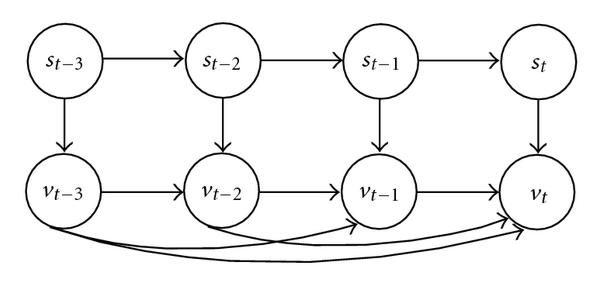
\includegraphics[width=0.6\linewidth]{bayes-dyn}
\end{center}
\end{frame}

\begin{frame}{Réseaux Bayésiens}{Utilisation}
\begin{itemize}
\item Inférence : obtenir la probabilité d'un ensemble de variables $R$
	étant donné la valeur des variables $C$ ;
	\begin{itemize}
	\item $P(a) + P(\overline{a}) = 1$
	\item $P(a \wedge b) = P(a) \times P(b | a)$
	\item $P(a | b) = \frac{P(b | a) \times P(a)}{P(b)}$ (règle de Bayes)
	\end{itemize}
\item Apprentissage : estimer la structure (graphe) et les paramètres (probabilités) du modèle
	à partir de données statistiques $D$.
\end{itemize}
\end{frame}

\begin{frame}{Réseaux Bayésiens}{Exemple}
\begin{itemize}
\item Je souhaite acheter une voiture modèle $X$ ;
\item AutoPlus indique que 30\% ont des problèmes de transmission ;
\item Je peux faire essayer une voiture par un ami mécano :
	\begin{itemize}
	\item Il reconnait $90\%$ des voitures défectueuses ;
	\item Il reconnait $80\%$ des voitures non défectueuses.
	\end{itemize}
\end{itemize}
\begin{itemize}
\item Questions :
	\begin{itemize}
	\item Probabilité d'acheter une voiture non défectueuse
	sachant que le diagnostic la reconnait comme non défectueuse ?
	\item Probabilité d'acheter une voiture non défectueuse (sans diagnostic) ?
	\item Probabilité d'acheter une voiture non défectueuse
	sachant que le diagnostic la reconnait comme défectueuse ?
	\end{itemize}
\end{itemize}
\end{frame}

%%%%% SYSTEMES HYBRIDES %%%%%
\section{Systèmes hybrides}

\begin{frame}
\tableofcontents[currentsection,hideothersubsections]
\end{frame}

\subsection{Automates hybrides}
\begin{frame}{Automates hybrides (Alur {\it et al.}, 1993)}
\begin{center}
\begin{tikzpicture}[node distance=6cm]
\node[state, initial] (off) {$\begin{array}{c}Off\\\dot{x} = -0.1\, x\\x \geq 18\end{array}$};%
\node[state] (on) [right of=off] {$\begin{array}{c}On\\\dot{x} = 5-0.1\, x\\x \leq 22\end{array}$};
\path[->] (off) edge[bend left] node {$x < 19$} (on);
\path[->] (on) edge[bend left] node {$x > 21$} (off);
\end{tikzpicture}\\
\small Automate hybride d'un thermostat
\end{center}
\end{frame}

\begin{frame}{Automates hybrides}
\begin{itemize}
\item Mesure \structure{numérique} $\rightarrow$ vecteur d'état du système,
\item Technique de filtrage numérique,
\item Situation : état de l'automate
\item[$\Longrightarrow$] Estimation de mode.
\end{itemize}
\begin{itemize}
\item Automates hybrides probabilistes + filtres de Kalman (Hofbaur et Williams, 2002),
\item Automates hybrides + filtrage particulaire (Koutsoukos {\it et al.}, 2003).
\end{itemize}
\end{frame}

\begin{frame}{Automates hybrides}{Filtrage particulaire}
%% L'automate
\begin{tikzpicture}[scale=0.5,transform shape,overlay]
\node[state, color=blue] (q_off) {$q_0$};
\node[state, color=red] (q_on) [below of=q_off] {$q_1$};
\node[state, failure] (q_failed) [right of=q_off] {$q_2$};
\path[->] (q_off) edge[loop left] ()
		edge (q_failed)
		edge[bend left] (q_on)
	(q_on) edge[loop left] ()
		edge[bend left] (q_off)
		edge[bend left] (q_failed)
	(q_failed) edge[loop right] ()
		edge[bend left] (q_on);
\end{tikzpicture}
\begin{center}
%% Les particules
\shorthandoff{:}
\begin{tikzpicture}[domain=-0.5:9,z={(1,0,0)},x={(0,0.6,0.6)}]
%% Axe
\draw[->] (0,0,0) -- (9,0,0);
\draw[->] (0,0,0) -- (0,2,0);
\draw[->] (0,0,0) -- (0,0,10) node[right] {$t$};
%% Indices
\draw (0,0,0) node[below] {$0$};
%% Plot Init
\path[draw, color=green, overlay]<2-> plot [id=exp,smooth] function{2*exp(-(x-2)*(x-2)/2) + exp(-(x-6)*(x-6)/2)};
%% Particules
\foreach \p in {6.5, 6.2, 5.5, 5, 3.5, 2.7, 2.2, 2.1, 1.9, 1}
	\path[draw, color=blue, thick, ->, overlay]<3-> (\p, 0) -- (\p, 1);
%% Pred automate
\foreach \p in {6.5, 6.2, 5.5, 5}
	\path[shade, shading=axis, very thick, left color=blue,right color=red, middle color=blue!30!red, overlay]<4-> (\p, 0, 0) rectangle +(0.01, 0, 1.5);
\foreach \p in {6.5, 6.2, 5.5, 5}
	\path[draw, thick, color=red, ->, overlay]<4-> (\p, 0, 1.5) -- (\p, 1, 1.5);
\foreach \p in {3.5, 2.7, 2.2, 2.1, 1.9, 1}
	\path[draw, color=blue, thick, ->, overlay]<4-> (\p, 0, 0) -- (\p, 0, 1.5) -- (\p, 1, 1.5);
%% Pred continue
\foreach \p/\d in {6.5/0.2, 6.2/0.3, 5.5/-0.6, 5/0.6}
	\path[draw, color=red, thick, ->, overlay]<5-> (\p, 0, 1.5) -- ++(\d, 0, 1.5) -- +(0, 1, 0);
\foreach \p/\d in {3.5/0.9, 2.7/0.3, 2.2/0.2, 2.1/1.1, 1.9/1.8, 1/0.3}
	\path[draw, color=blue, thick, ->, overlay]<5-> (\p, 0, 1.5) -- ++(\d, 0, 1.5) -- +(0, 1, 0);
%% Plot Observation
\path[draw, ->, overlay]<6-> (0, 0, 4.5) -- +(9, 0, 0);
\path[draw, color=green, shift={(0,0,4.5)}, overlay]<6-> plot[id=exp,smooth] function{2*exp(-(x-4)*(x-4)/2)};
\path[draw, overlay]<6-> (0,0,4.5) node[below] {$1$};
%% Ponderation
\foreach \p/\d/\w in {6.5/0.2/0.1, 6.2/0.3/0.1, 5.5/-0.6/1.3, 5/0.6/0.5}
	\path[draw, color=red, thick, ->, overlay]<7-> (\p, 0, 3) ++(\d, 0, 0) -- ++(0, 0, 1.5) -- +(0, \w, 0);
\foreach \p/\d/\w in {3.5/0.9/1.9, 2.7/0.3/1.0, 2.2/0.2/0.4, 2.1/1.1/1.2, 1.9/1.8/1.8, 1/0.3/0.1}
	\path[draw, color=blue, thick, ->, overlay]<7-> (\p, 0, 3) ++(\d, 0, 0) -- ++(0, 0, 1.5) -- +(0, \w, 0);
%% Resampling
\foreach \p/\d in {5/0.6}
	\path[shade, shading=axis, thick, left color=red,right color=blue, middle color=blue!30!red, overlay]<8-> (\p, 0, 4.5) ++(\d, 0, 0) rectangle +(0.01, 0, 1.5);
\foreach \p/\d in {5/0.6}
	\path[draw, color=blue, thick, ->, overlay]<8-> (\p, 0, 4.5) ++(\d, 0, 1.5) -- +(0, 1, 0);
\foreach \p/\d/\w in {3.5/0.9/0, 2.7/0.3/0.05, 2.2/0.2/0.05, 2.1/1.1/0.05, 1.9/1.8/0.05, 2.7/0.3/-0.05, 2.2/0.2/-0.05, 2.1/1.1/-0.05, 1.9/1.8/-0.05}
	\path[draw, color=blue, thick, ->, overlay]<8-> (\p, 0, 4.5) ++(\d, 0, 0) -- ++(\w, 0, 1.5) -- +(0, 1, 0);

\end{tikzpicture}
\end{center}
\end{frame}

%%%%% RESEAUX DE PETRI %%%%%
\subsection{Réseaux de Petri hybrides}
\begin{frame}{Réseaux de Petri particulaires (Lesire et Tessier, 2005)}
\begin{columns}
\begin{column}{0.6\linewidth}
\begin{itemize}[<+->]
\item RdP $\rightarrow$ dynamique discrète
\item Marquage $\rightarrow$ état discret
\item Jeton numérique $\rightarrow$ état hybride
\item Eq. Dif. $\rightarrow$ dynamique hybride
\item Particules $\rightarrow$ incertitude hybride
\item Macro-marquage $\rightarrow$ incertitude symbolique
\end{itemize}
\end{column}
\begin{column}{0.4\linewidth}
\begin{tikzpicture}[scale=0.8, transform shape, node distance=35pt]

\node[place, label=right:OPDES] (p0) at (3, 7) {};
\node[place, label=right:ALT] (p1) at (3, 5) {};
\node[place, label=right:ALT] (p2) at (3, 3) {};
\node[place, label=right:LOC] (p3) at (3, 1) {};
\node[place] (p6) at (0, 6) {};
\node[place] (p7) at (0, 2) {};
\node[transition] (t0) at (3, 6) {};
\node[transition, label=left:$d < 10$] (t1) at (1.5, 4) {};
\node[transition] (t2) at (3, 2) {};
\node[transition, label=left:$r. 145$] (t3) at (1.5, 0) {};
%% Post
\foreach \t/\p in {t0/p1,t1/p2,t1/p7,t2/p3}
	\path (\t) edge[post] (\p);
%% Pre
\foreach \p/\t in {p0/t0,p1/t1,p6/t1,p2/t2,p3/t3,p7/t3}
	\path (\t) edge[pre] (\p);
%% Animation
\path[overlay]<1-3|handout:0> node[left of=p6] {Descente};
\path[overlay]<1-3|handout:0> node[left of=p7] {Palier};
\path[overlay]<4-> node[left of=p6] {$\dot{z} = v_z$};
\path[overlay]<4-> node[left of=p7] {$\dot{z} = 0$};
%% Marquage
\path[overlay]<2-> node[place, tokens=1] at (3, 7) {};
\path[overlay]<6-> node[place, tokens=1] at (3, 5) {};
\path[overlay]<2|handout:0> node[place, tokens=1] at (0, 6) {};
\path[overlay]<3-4|handout:0> node[place] at (0, 6) {$\mathbf{X}$};
\path[overlay]<5-> node[place, tokens=5] at (0, 6) {};
\end{tikzpicture}
\end{column}
\end{columns}
\end{frame}

\begin{frame}{Réseaux de Petri particulaires}
\begin{columns}
\begin{column}{0.6\linewidth}
\begin{tikzpicture}[domain=-0.5:9,z={(0.5,0,0)},x={(0,0.6,1.2)}]
%% Axe
\draw[->] (0,0,0) -- (9,0,0);
\draw[->] (0,0,0) -- (0,2,0);
\draw[->] (0,0,0) -- (0,0,10) node[right] {$t$};
%% Indices
\draw (0,0,0) node[below] {$0$};
%% Plot Init
\path[draw, color=green, overlay]<2-> plot [id=exp,smooth] function{2*exp(-(x-2)*(x-2)/2) + exp(-(x-6)*(x-6)/2)};
%% Particules
\foreach \p in {6.5, 6.2, 5.5, 5, 3.5, 2.7, 2.2, 2.1, 1.9, 1}
	\path[draw, color=blue, thick, ->, overlay]<3-> (\p, 0) -- (\p, 1);
%% Pred automate
\foreach \p in {6.5, 6.2, 5.5, 5}
	\path[shade, shading=axis, very thick, left color=blue,right color=red, middle color=blue!30!red, overlay]<4-> (\p, 0, 0) rectangle +(0.01, 0, 1.5);
\foreach \p in {6.5, 6.2, 5.5, 5}
	\path[draw, thick, color=red, ->, overlay]<4-> (\p, 0, 1.5) -- (\p, 1, 1.5);
\foreach \p in {3.5, 2.7, 2.2, 2.1, 1.9, 1}
	\path[draw, color=blue, thick, ->, overlay]<4-> (\p, 0, 0) -- (\p, 0, 1.5) -- (\p, 1, 1.5);
%% Pred continue
\foreach \p/\d in {6.5/0.2, 6.2/0.3, 5.5/-0.6, 5/0.6}
	\path[draw, color=red, thick, ->, overlay]<5-> (\p, 0, 1.5) -- ++(\d, 0, 1.5) -- +(0, 1, 0);
\foreach \p/\d in {3.5/0.9, 2.7/0.3, 2.2/0.2, 2.1/1.1, 1.9/1.8, 1/0.3}
	\path[draw, color=blue, thick, ->, overlay]<5-> (\p, 0, 1.5) -- ++(\d, 0, 1.5) -- +(0, 1, 0);
%% Plot Observation
\path[draw, ->, overlay]<6-> (0, 0, 4.5) -- +(9, 0, 0);
\path[draw, color=green, shift={(0,0,4.5)}, overlay]<6-> plot[id=exp,smooth] function{2*exp(-(x-4)*(x-4)/2)};
\path[draw, overlay]<6-> (0,0,4.5) node[below] {$1$};
%% Ponderation
\foreach \p/\d/\w in {6.5/0.2/0.1, 6.2/0.3/0.1, 5.5/-0.6/1.3, 5/0.6/0.5}
	\path[draw, color=red, thick, ->, overlay]<7-> (\p, 0, 3) ++(\d, 0, 0) -- ++(0, 0, 1.5) -- +(0, \w, 0);
\foreach \p/\d/\w in {3.5/0.9/1.9, 2.7/0.3/1.0, 2.2/0.2/0.4, 2.1/1.1/1.2, 1.9/1.8/1.8, 1/0.3/0.1}
	\path[draw, color=blue, thick, ->, overlay]<7-> (\p, 0, 3) ++(\d, 0, 0) -- ++(0, 0, 1.5) -- +(0, \w, 0);
%% Resampling
\foreach \p/\d in {5/0.6}
	\path[shade, shading=axis, thick, left color=red,right color=blue, middle color=blue!30!red, overlay]<8-> (\p, 0, 4.5) ++(\d, 0, 0) rectangle +(0.01, 0, 1.5);
\foreach \p/\d in {5/0.6}
	\path[draw, color=blue, thick, ->, overlay]<8-> (\p, 0, 4.5) ++(\d, 0, 1.5) -- +(0, 1, 0);
\foreach \p/\d/\w in {3.5/0.9/0, 2.7/0.3/0.05, 2.2/0.2/0.05, 2.1/1.1/0.05, 1.9/1.8/0.05, 2.7/0.3/-0.05, 2.2/0.2/-0.05, 2.1/1.1/-0.05, 1.9/1.8/-0.05}
	\path[draw, color=blue, thick, ->, overlay]<8-> (\p, 0, 4.5) ++(\d, 0, 0) -- ++(\w, 0, 1.5) -- +(0, 1, 0);

\end{tikzpicture}
\end{column}
\begin{column}{0.4\linewidth}
\begin{tikzpicture}[scale=0.8, transform shape]

\node[place, label=right:OPDES] (p0) at (3, 7) {};
\node[place, label=right:ALT] (p1) at (3, 5) {};
\node[place, label=right:ALT] (p2) at (3, 3) {};
\node[place, label=right:LOC] (p3) at (3, 1) {};
\node[place] (p6) at (0, 6) {};
\node[place] (p7) at (0, 2) {};
\node[transition] (t0) at (3, 6) {};
\node[transition, label=left:$d < 10$] (t1) at (1.5, 4) {};
\node[transition] (t2) at (3, 2) {};
\node[transition, label=left:$r. 145$] (t3) at (1.5, 0) {};
%% Post
\foreach \t/\p in {t0/p1,t1/p2,t1/p7,t2/p3}
	\path (\t) edge[post] (\p);
%% Pre
\foreach \p/\t in {p0/t0,p1/t1,p6/t1,p2/t2,p3/t3,p7/t3}
	\path (\t) edge[pre] (\p);
%% Places symb.
\path[overlay]<1-8|handout:0> node[place, tokens=1] at (3, 7) {};
\path[overlay]<4-> node[place, tokens=1] at (3, 5) {};
\path[overlay]<4-> node[place, tokens=1] at (3, 3) {};
%% Places num.
\path[overlay]<1-2|handout:0> node[place, tokens=1] at (0, 6) {};
\path[overlay]<3|handout:0> node[place, structured tokens={10}] at (0, 6) {};
\path[overlay]<4-7|handout:0> node[place, tokens=6] at (0, 6) {};
\path[overlay]<4-7|handout:0> node[place, tokens=4] at (0, 2) {};
\path[overlay]<8-9> node[place, structured tokens={9}] at (0, 6) {};
\path[overlay]<8-9> node[place, tokens=1] at (0, 2) {};
\end{tikzpicture}
\end{column}
\end{columns}
\end{frame}

\begin{frame}{Réseaux de Petri particulaires}
\begin{columns}
\begin{column}{0.6\linewidth}
\begin{itemize}
\item Modèle riche
\item Pas d'interaction continu/discret lors du recalage
\item[$\Longrightarrow$] détection d'incohérences
\end{itemize}
\end{column}
\begin{column}{0.4\linewidth}
\begin{tikzpicture}[scale=0.8, transform shape]

\node[place, label=right:OPDES] (p0) at (3, 7) {};
\node[place, label=right:ALT] (p1) at (3, 5) {};
\node[place, label=right:ALT] (p2) at (3, 3) {};
\node[place, label=right:LOC] (p3) at (3, 1) {};
\node[place] (p6) at (0, 6) {};
\node[place] (p7) at (0, 2) {};
\node[transition] (t0) at (3, 6) {};
\node[transition, label=left:$d < 10$] (t1) at (1.5, 4) {};
\node[transition] (t2) at (3, 2) {};
\node[transition, label=left:$r. 145$] (t3) at (1.5, 0) {};
%% Post
\foreach \t/\p in {t0/p1,t1/p2,t1/p7,t2/p3}
	\path (\t) edge[post] (\p);
%% Pre
\foreach \p/\t in {p0/t0,p1/t1,p6/t1,p2/t2,p3/t3,p7/t3}
	\path (\t) edge[pre] (\p);
\node[place, tokens=1] at (3, 7) {};
\node[place, tokens=1] at (0, 2) {};
\end{tikzpicture}
\end{column}
\end{columns}
\end{frame}

\begin{frame}{Réseaux de Petri particulaires}
\begin{itemize}
\item Places numériques, associées à des équations d'évolution (modes continus) ;
\item Places symboliques, associées à des configurations (modes discrets) ;
\item Transitions représentant les changements de mode, selon :
	\begin{itemize}
	\item l'évolution continue (gardes sur les paramètres du vecteur d'état) ;
	\item l'évolution discrète (actions / événements externes) ;
	\end{itemize}
\item Marquage hybride :
	\begin{itemize}
	\item jetons \structure{noirs} dans les places symboliques (modes discrets possibles du systèmes)
	\item \structure{particules} dans les places numériques (distribution sur le vecteur d'état)
	\end{itemize}
\end{itemize}
\end{frame}

\begin{frame}{Réseaux de Petri particulaires}
\begin{center}
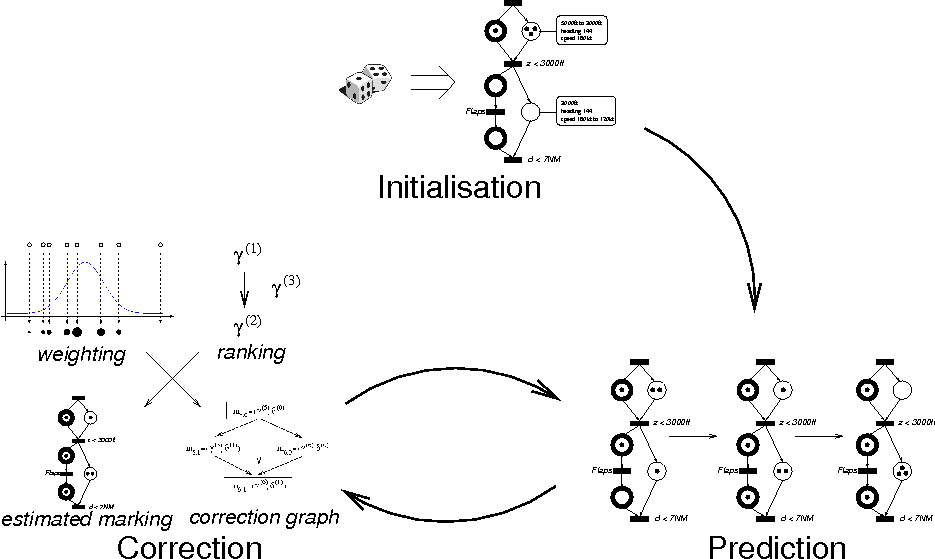
\includegraphics[width=0.8\linewidth]{estimation}
\end{center}
\end{frame}

\begin{frame}{Réseaux de Petri particulaires}
\begin{itemize}
\item $\frac{\text{nombre de particulares dans }p}{\text{nombre de particles}} = \frac{|\mathcal{M}(p)|}{N} = $
probabilité d'être dans le mode numérique associté à $p$
\item On agrège donc cette information, pour avoir :
	\begin{itemize}
	\item une proba pour chaque place numérique
	\item un classement pour chaque place symbolique
	\end{itemize}
\item On regarde le couple $(p, q)$ le plus vraissemblable :
$\longrightarrow$ est-il accessible depuis le marquage initial ?
\end{itemize}
\end{frame}

%%%%% GHOST %%%%%
\section{Suivi de  l'activité de pilotage}

\begin{frame}
\tableofcontents[currentsection,hideothersubsections]
\end{frame}

\subsection{Ghost}
\begin{frame}{Suivi de l'activité de pilotage (Dehais {\it et al.}, 2005)}
\begin{itemize}
\item Le système avion--pilote est \structure{hybride} :
	\begin{itemize}
	\item Dynamique continue de l'avion,
	\item Actions discrètes du pilote.
	\end{itemize}
\item Modélisation sous forme de \structure{réseau de Petri particulaire}
\item Intégration de mécanisme de détection de conflits
\end{itemize}
\end{frame}

\begin{frame}{Suivi de l'activité de pilotage}
\begin{columns}
\begin{column}{0.4\linewidth}
	\begin{tikzpicture}[scale=0.8, transform shape, node distance=35pt]
	
\node[place, label=right:OPDES] (p0) at (3, 7) {};
\node[place, label=right:ALT] (p1) at (3, 5) {};
\node[place, label=right:ALT] (p2) at (3, 3) {};
\node[place, label=right:LOC] (p3) at (3, 1) {};
\node[place] (p6) at (0, 6) {};
\node[place] (p7) at (0, 2) {};
\node[transition] (t0) at (3, 6) {};
\node[transition, label=left:$d < 10$] (t1) at (1.5, 4) {};
\node[transition] (t2) at (3, 2) {};
\node[transition, label=left:$r. 145$] (t3) at (1.5, 0) {};
%% Post
\foreach \t/\p in {t0/p1,t1/p2,t1/p7,t2/p3}
	\path (\t) edge[post] (\p);
%% Pre
\foreach \p/\t in {p0/t0,p1/t1,p6/t1,p2/t2,p3/t3,p7/t3}
	\path (\t) edge[pre] (\p);
	\end{tikzpicture}
\end{column}
\begin{column}{0.6\linewidth}
\begin{itemize}
\item Modélisation de la trajectoire avion
\item De sa configuration (volets, train\dots)
\item Du comportement du PA (modes, transitions)
\item Des actions pilotes (en lien avec PA / conf.)
\end{itemize}
\vspace{1cm}
\begin{itemize}
\item Détection d'\structure{incohérences}
\item Identification de modes \structure{défaillants}
\end{itemize}
\end{column}
\end{columns}
\end{frame}

\begin{frame}{Suivi de l'activité de pilotage}
\begin{center}
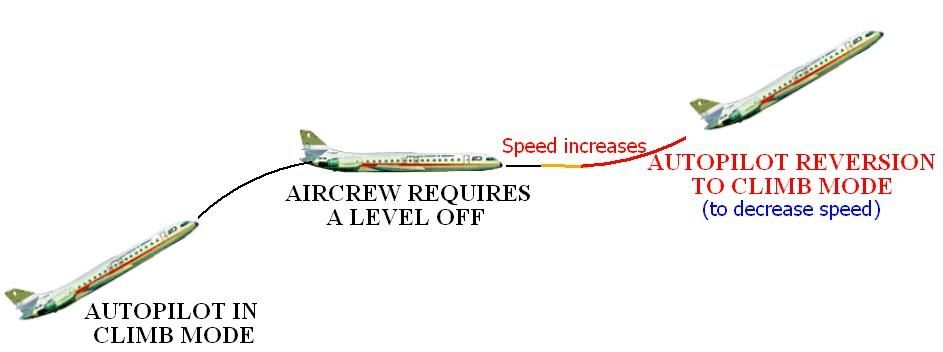
\includegraphics[width=0.8\linewidth]{LevelOff}
\end{center}
\end{frame}

\begin{frame}{Suivi de l'activité de pilotage}
\begin{center}
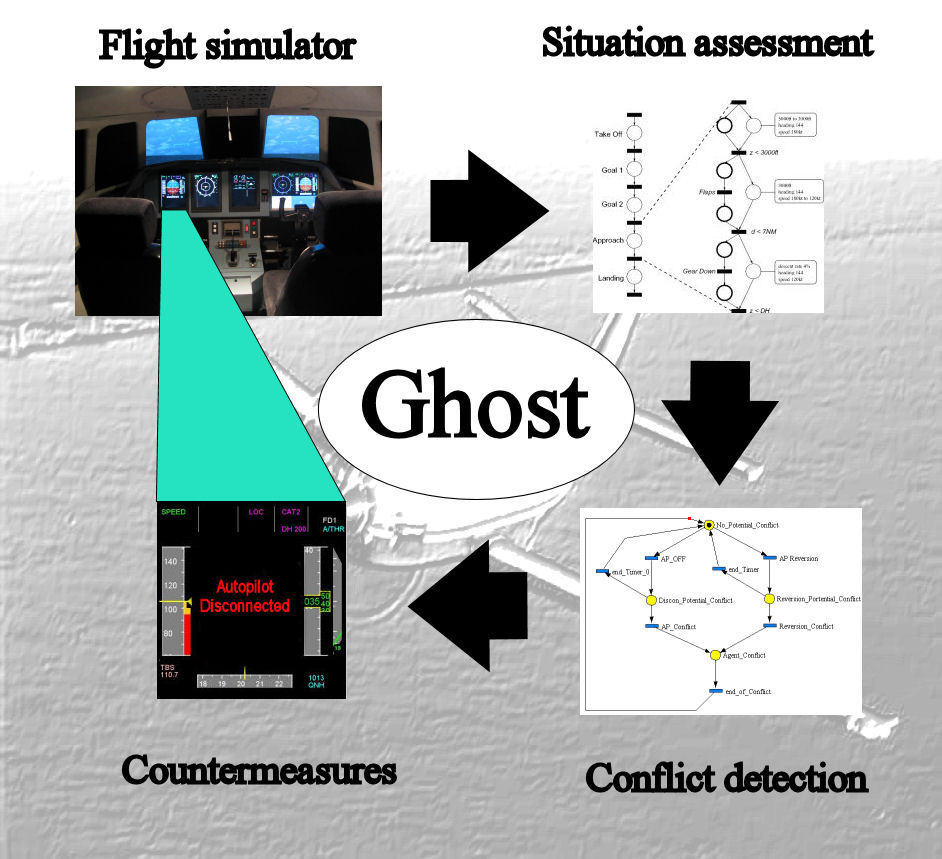
\includegraphics[width=0.6\linewidth]{ghost_pp}
\end{center}
\end{frame}

\begin{frame}{Suivi de l'activité de pilotage}
\begin{columns}
\begin{column}{0.5\linewidth}
	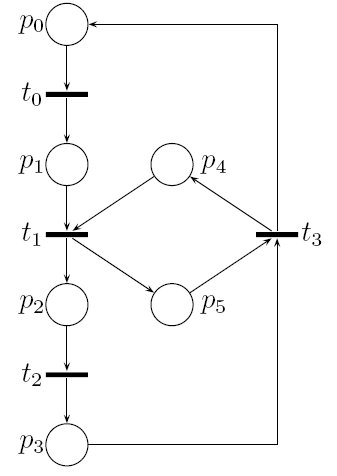
\includegraphics[width=0.6\linewidth]{rev-petri}
\end{column}
\begin{column}{0.5\linewidth}
	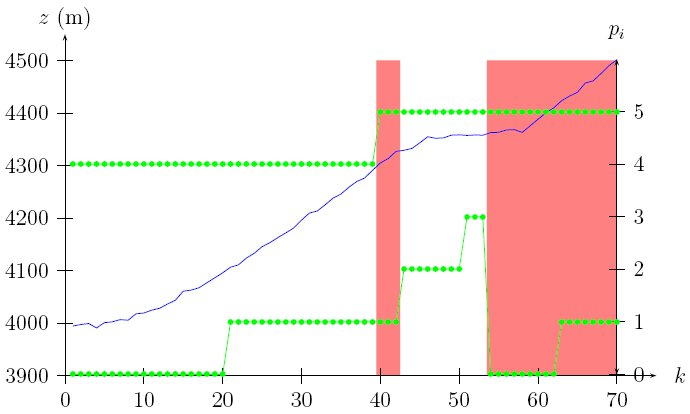
\includegraphics[width=0.9\linewidth]{reversion-z}
\end{column}
\end{columns}
\begin{center}
\small Estimation et détection d'incohérences\\
\alert{$\rightarrow$ incohérence détectée à partir de $t = 60$}
\end{center}
\end{frame}

\begin{frame}{Suivi de l'activité de pilotage}{Conclusion}
\begin{itemize}
\item Formalisme pour le suivi du comportement avion--pilote
\item Détection d'incohérences $\rightarrow$ \structure{conflits}
\item \structure{Prédiction} de conflits
\item Utilisation de \structure{données physio} pour l'{\it état} du pilote
\item Assistance au pilotage (présentation des infos estimation)
\item Automatisation (partielle) de certaines procédures
\end{itemize}
\end{frame}

\end{document}
